\documentclass[12pt,a4paper]{report}

\usepackage[a4paper,top=35mm,bottom=25mm,left=38.1mm,right=25.4mm]{geometry}
\usepackage[T1]{fontenc}
\usepackage[utf8]{inputenc}
\usepackage{mathptmx}
\usepackage[scaled=0.92]{helvet}
\usepackage{courier}
\usepackage{setspace}
\onehalfspacing
\usepackage{amsmath,amssymb}
\usepackage{graphicx}
\usepackage{booktabs}
\usepackage{array}
\usepackage{tabularx}
\usepackage{tikz}
\usetikzlibrary{shapes.geometric, arrows.meta, positioning, fit, calc, backgrounds}
\usepackage{algorithm}
\usepackage{algorithmic}
\usepackage[hidelinks,plainpages=false,pdfpagelabels]{hyperref}
\usepackage{titlesec}
\usepackage{caption}

\titleformat{\chapter}[display]
  {\normalfont\Large\bfseries\centering}{\MakeUppercase{\chaptertitlename}\ \thechapter}{10pt}{\Large\MakeUppercase}
\titlespacing*{\chapter}{0pt}{-10pt}{20pt}
\titleformat{\section}{\normalfont\large\bfseries}{\thesection}{1em}{}
\titlespacing*{\section}{0pt}{16pt plus 3pt minus 2pt}{6pt plus 2pt minus 2pt}
\titleformat{\subsection}{\normalfont\normalsize\bfseries}{\thesubsection}{1em}{}
\titlespacing*{\subsection}{0pt}{12pt plus 2pt minus 2pt}{4pt plus 2pt minus 2pt}

\setlength{\parindent}{20pt}
\setlength{\parskip}{4pt plus 1.5pt minus 1pt}
\setcounter{tocdepth}{2}
\pagestyle{plain}

\definecolor{cBlue}{HTML}{2563EB}
\definecolor{cBlueBg}{HTML}{DBEAFE}
\definecolor{cTeal}{HTML}{0D9488}
\definecolor{cTealBg}{HTML}{CCFBF1}
\definecolor{cAmber}{HTML}{D97706}
\definecolor{cAmberBg}{HTML}{FEF3C7}
\definecolor{cViolet}{HTML}{7C3AED}
\definecolor{cVioletBg}{HTML}{EDE9FE}
\definecolor{cRose}{HTML}{E11D48}
\definecolor{cRoseBg}{HTML}{FFE4E6}
\definecolor{cGreen}{HTML}{16A34A}
\definecolor{cGreenBg}{HTML}{DCFCE7}
\definecolor{cSlate}{HTML}{334155}

\tikzset{
  stage/.style={draw=cBlue, line width=0.7pt, rounded corners=3pt, align=center,
                font=\footnotesize, inner sep=5pt, minimum height=9mm, fill=cBlueBg, text=cSlate},
  sBlue/.style={draw=cBlue, fill=cBlueBg, text=cSlate},
  sTeal/.style={draw=cTeal, fill=cTealBg, text=cSlate},
  sAmber/.style={draw=cAmber, fill=cAmberBg, text=cSlate},
  sViolet/.style={draw=cViolet, fill=cVioletBg, text=cSlate},
  sRose/.style={draw=cRose, fill=cRoseBg, text=cSlate},
  sGreen/.style={draw=cGreen, fill=cGreenBg, text=cSlate},
  farrow/.style={-{Latex[length=2.4mm]}, line width=0.9pt, draw=cSlate},
}

\begin{document}
\pagenumbering{alph}

% ===================== TITLE =====================
\thispagestyle{empty}
\begin{center}
    \vspace*{2mm}
    {\Large\bfseries How Robust is Structure-Aware Retrieval? Quantifying and Mitigating the Effect of Document-Structure Errors in Retrieval-Augmented Generation\par}
    \vspace{6mm}
    {\large Minor Project (IT897) Report\par}
    \vspace{3mm}
    {\normalsize Submitted in partial fulfillment of the requirements for the degree of\par}
    \vspace{1.5mm}
    {\large MASTER OF TECHNOLOGY\par}
    \vspace{1mm}{\normalsize in\par}\vspace{1mm}
    {\large INFORMATION TECHNOLOGY\par}
    \vspace{5mm}{\normalsize by\par}\vspace{1.5mm}
    {\large\bfseries KSHITIJ KHEDE\par}
    \vspace{1mm}{\large\bfseries (252IT010)\par}
    \vspace{5mm}{\large\itshape under the guidance of\par}\vspace{1.5mm}
    {\large\bfseries Prof. ANANTHANARAYANA V. S.\par}
    \vspace{6mm}
    
\includegraphics[width=32mm]{images/nitk_logo_report_pdf.jpeg}
    \vspace{6mm}
    {\large DEPARTMENT OF INFORMATION TECHNOLOGY\par}\vspace{1mm}
    {\large NATIONAL INSTITUTE OF TECHNOLOGY KARNATAKA\par}\vspace{1mm}
    {\large SURATHKAL, MANGALURU -- 575025\par}\vspace{1.5mm}
    {\large September 2026\par}
\end{center}
\clearpage

% ===================== DECLARATION =====================
\thispagestyle{empty}
\begin{center}
\setlength{\fboxsep}{8mm}\setlength{\fboxrule}{0.8pt}
\noindent\fbox{%
\begin{minipage}{\dimexpr\textwidth-2\fboxsep-2\fboxrule-3pt\relax}
\vspace{2mm}\begin{center}{\Large\bfseries DECLARATION}\end{center}\vspace{8mm}
\noindent I hereby declare that the report of the P.G. Minor Project (IT897) work entitled
\textbf{``How Robust is Structure-Aware Retrieval? Quantifying and Mitigating the Effect of
Document-Structure Errors in Retrieval-Augmented Generation''}, submitted to the National
Institute of Technology Karnataka, Surathkal, in partial fulfillment of the requirements for
the award of the degree of \textbf{Master of Technology in Information Technology}, is a bona
fide record of the work carried out by me. The material in this report has not been submitted
to any university or institution for the award of any degree.
\vspace{18mm}
\begin{flushright}\textbf{Kshitij Khede (252IT010)} \\ Dept. of Information Technology \\ NITK Surathkal, Mangaluru\end{flushright}
\vspace{8mm}\noindent Place: NITK, Surathkal \\ Date: September 2026 \vspace{2mm}
\end{minipage}}
\end{center}
\clearpage

% ===================== CERTIFICATE =====================
\thispagestyle{empty}
\begin{center}
\setlength{\fboxsep}{8mm}\setlength{\fboxrule}{0.8pt}
\noindent\fbox{%
\begin{minipage}{\dimexpr\textwidth-2\fboxsep-2\fboxrule-3pt\relax}
\vspace{2mm}\begin{center}{\Large\bfseries CERTIFICATE}\end{center}\vspace{8mm}
\noindent This is to certify that the P.G. Minor Project (IT897) work entitled
\textbf{``How Robust is Structure-Aware Retrieval? Quantifying and Mitigating the Effect of
Document-Structure Errors in Retrieval-Augmented Generation''}, submitted by
\textbf{Kshitij Khede (252IT010)} as the record of the work carried out by him, is accepted as
the P.G. Minor Project (IT897) work report submission in partial fulfillment of the requirements
for the award of the degree of \textbf{Master of Technology in Information Technology} in the
Department of Information Technology, NITK Surathkal, India. Duration of this minor project
(IT897) is from JUNE 01, 2026 to AUGUST 15, 2026.
\vspace{25mm}
\begin{center}\textbf{Prof. ANANTHANARAYANA V. S.} \\[2mm]{\normalsize (Signature of the Guide with Date and Seal)}\end{center}
\vspace{6mm}
\end{minipage}}
\end{center}
\clearpage

% ===================== ACKNOWLEDGEMENT =====================
\thispagestyle{empty}
\begin{center}{\Large\bfseries ACKNOWLEDGEMENT}\end{center}\vspace{8mm}
\noindent I am thankful to my guide, \textbf{Prof. Ananthanarayana V. S.}, for his guidance and
feedback throughout this minor project. His questions on whether the recovered document structure
can be trusted directly shaped the research direction of this work.
\vspace{3mm}\noindent
I also thank the Department of Information Technology, NITK Surathkal, for the facilities and
academic environment provided for this project.
\vspace{25mm}\begin{flushright}\textbf{Kshitij Khede}\end{flushright}
\clearpage

% ===================== ABSTRACT =====================
\pagenumbering{roman}\setcounter{page}{1}
\begin{center}{\Large\bfseries ABSTRACT}\end{center}\vspace{2mm}
\begin{spacing}{1.10}
\noindent
Retrieval-Augmented Generation (RAG) increasingly represents documents not as flat text chunks
but as a hierarchy of sections, so that a retriever can attach the surrounding structural context
of a passage. A growing family of systems --- RAPTOR, TreeRAG, HiChunk, BookRAG and layout-aware
retrievers --- build such a hierarchy and then \emph{assume it is correct}. Real documents, however,
are parsed imperfectly: multi-column pages are mis-ordered and section headings are mis-detected.
This project asks, for the first time, how sensitive structure-aware retrieval is to such errors,
whether the errors can be detected from a per-node confidence signal, and whether they can be
repaired at inference time without re-parsing.

The recovered hierarchy is treated as an instrument, and two controllable error sources are
injected: reading-order noise ($\rho$) and heading-number dropout ($\delta$). Structural fidelity
is measured with three retrieval-relevant, model-free metrics: Parent-Assignment Accuracy (PAA),
Ancestor-Path Accuracy (APA, the ancestor context a hierarchical retriever would attach), and
Ancestor-Context Precision (ACP). A confidence-gated repair step reattaches low-confidence nodes
to a safe structural prior.

On a corpus of eleven research-paper PDFs (five seeds per setting), reading-order noise is almost
harmless (APA $96.8\% \rightarrow 96.4\%$ at $50\%$ noise) because numbering-primary attachment is
inherently order-robust, whereas heading-number loss degrades structure steadily (PAA
$97.7\%\rightarrow 92.7\%$, APA $96.8\%\rightarrow 89.2\%$ at $50\%$ loss). Attachment errors occur
in lower-confidence nodes (correct $0.61$ vs.\ wrong $0.55$; point-biserial $r=+0.16$), and
confidence-gated repair recovers part of the loss (APA $92.8\%\rightarrow 93.3\%$). The results
give the first robustness characterisation of structure-aware retrieval and an inference-time
mitigation, and they identify learned structural confidence as the key lever for future work.

\vspace{3mm}\noindent\textbf{Keywords:} Retrieval-Augmented Generation; Structure-Aware Retrieval;
Robustness; Document Structure; Confidence Estimation; Ancestor Context.
\end{spacing}
\clearpage

% ===================== FRONT LISTS =====================
\tableofcontents\clearpage
\phantomsection\addcontentsline{toc}{chapter}{LIST OF FIGURES}\listoffigures\clearpage
\phantomsection\addcontentsline{toc}{chapter}{LIST OF TABLES}\listoftables\clearpage
\phantomsection\addcontentsline{toc}{chapter}{ABBREVIATIONS}
\begin{center}{\Large\bfseries ABBREVIATIONS}\end{center}\vspace{6mm}
\noindent\begin{tabularx}{\textwidth}{@{} >{\bfseries}p{3.0cm} X @{}}
\toprule \textbf{Abbreviation} & \textbf{Full Form} \\ \midrule
RAG & Retrieval-Augmented Generation \\
PDF & Portable Document Format \\
PAA & Parent-Assignment Accuracy \\
APA & Ancestor-Path Accuracy \\
ACP & Ancestor-Context Precision \\
PRE & Parent Ranking Engine \\
KCE & Knowledge Confidence Estimation \\
CPG & Candidate Parent Generation \\
TF--IDF & Term Frequency--Inverse Document Frequency \\
DFS & Depth-First Search \\
LLM & Large Language Model \\
OCR & Optical Character Recognition \\ \bottomrule
\end{tabularx}\clearpage

% ===================== CH1 INTRODUCTION =====================
\pagenumbering{arabic}\setcounter{page}{1}
\chapter{Introduction}

\section{Background}
Large Language Models answer fluently but can state untrue facts and cannot see knowledge created
after training. Retrieval-Augmented Generation (RAG) addresses both by retrieving relevant text
from an external store at query time and giving it to the model as
context~\cite{lewis2020rag,guu2020realm}. The quality of a RAG answer therefore depends heavily on
what is retrieved, which in turn depends on how the source document is represented before retrieval.

Early RAG splits a document into flat, fixed-size chunks~\cite{borgeaud2022retro,izacard2023atlas}.
Recent systems instead represent a document as a \emph{hierarchy} --- title, sections, subsections
--- and retrieve along it, so that when a passage is returned its ancestor sections are attached as
context~\cite{sarthi2024raptor,tao2025treerag,lu2026hichunk}. This is now a large and active family
of ``structure-aware'' methods.

\section{The Gap: Structure is Assumed Correct}
Structure-aware systems all share one assumption: that the recovered hierarchy is correct. In
practice the hierarchy is produced by an imperfect parser. Two failures are common on real PDFs:
(i) \textbf{reading-order errors}, where a multi-column page is read across columns, and (ii)
\textbf{heading-detection errors}, where a section number is missed or garbled. When a section is
attached to the wrong parent, a hierarchical retriever silently attaches the \emph{wrong ancestor
context} to the query --- with no error flag. No prior work quantifies how damaging this is, whether
it can be predicted, or whether it can be repaired.

\section{Motivation}
If structure-aware retrieval is fragile to ordinary parsing noise, then reported gains on clean
documents may not transfer to real ones, and the errors are dangerous precisely because they are
silent. Conversely, if the representation already carries a usable confidence signal, that signal
could be used to detect and repair weak structure cheaply, at inference time. Establishing which of
these holds is a prerequisite for trusting structure-aware RAG in practice.

\section{Scope and Contributions}
This work studies robustness of the \emph{structural representation} that feeds a hierarchical
retriever; it does not train or evaluate an end-to-end generator (that is left to future work). The
contributions are:
\begin{enumerate}
  \item A controlled perturbation framework that injects two realistic, independently tunable
  structural error sources (reading-order noise $\rho$, heading-number dropout $\delta$) into a
  layout-aware document pipeline.
  \item Three model-free, retrieval-relevant fidelity metrics --- PAA, Ancestor-Path Accuracy (APA),
  and Ancestor-Context Precision (ACP) --- that measure the context a hierarchical retriever would
  attach.
  \item The first empirical robustness characterisation of structure-aware retrieval, including the
  finding that numbering-primary attachment is inherently robust to reading-order errors while being
  vulnerable to heading-number loss.
  \item A confidence-gated repair mechanism that reattaches low-confidence nodes at inference time,
  with an ablation quantifying its effect.
\end{enumerate}

\section{Organisation of the Report}
Chapter~2 reviews related work and states the problem and objectives. Chapter~3 describes the
instrument, the perturbation model, the metrics, and the repair. Chapter~4 reports the experiments
and results. Chapter~5 concludes and lists future work.

% ===================== CH2 LITERATURE REVIEW =====================
\chapter{Literature Review}
This chapter reviews retrieval and document-structure methods related to this project.
Table~\ref{tab:lit} summarises the most relevant works and the gap each leaves open.

\begin{table}[!htbp]\centering
\caption{Summary of the literature survey for the most relevant related works.}
\label{tab:lit}\renewcommand{\arraystretch}{1.3}{\small
\begin{tabularx}{\textwidth}{@{} >{\bfseries}p{2.6cm} p{2.6cm} X @{}}
\toprule Work & Category & Main idea and limitation \\ \midrule
Lewis et al.~\cite{lewis2020rag} & Flat RAG & Generator + dense passage retrieval; treats documents as flat passages. \\
Borgeaud et al.~\cite{borgeaud2022retro} & Flat RAG & Retrieval over trillions of tokens with fixed chunks; no document structure. \\
Sarthi et al.~\cite{sarthi2024raptor} & Tree RAG & Recursive clustering/summarisation tree; assumes clean inputs; no structural-error study. \\
Tao et al.~\cite{tao2025treerag} & Tree RAG & Tree-chunking along headings; needs correct heading markup; robustness untested. \\
Lu et al.~\cite{lu2026hichunk} & Tree RAG & Hierarchical chunking via fine-tuned LLM; evaluated on clean structure. \\
Zhang et al.~\cite{bookrag2025} & Hierarchical index & Tree + entity graph + agent for books; assumes reliable structure extraction. \\
Xu et al.~\cite{ladrag2025} & Layout-aware & Symbolic layout graph + agent for visually-rich docs; does not study parser-error robustness. \\
Wallat et al.~\cite{wallat2025faith} & Attribution & Shows RAG citations can be correct yet unfaithful; faithfulness under noise unsolved. \\
\bottomrule
\end{tabularx}}
\end{table}

\section{Flat and Adaptive Retrieval}
Lewis et al.~\cite{lewis2020rag} and Guu et al.~\cite{guu2020realm} connect a language model to a
document store; Borgeaud et al.~\cite{borgeaud2022retro} and Izacard et al.~\cite{izacard2023atlas}
scale and jointly train retrieval. Asai et al.~\cite{asai2024selfrag} make retrieval selective.
All operate over flat chunks and discard document structure.

\section{Structure-Aware and Hierarchical Retrieval}
Sarthi et al.~\cite{sarthi2024raptor} (RAPTOR) build a tree by clustering and summarising chunks;
Tao et al.~\cite{tao2025treerag} (TreeRAG) chunk along headings; Lu et al.~\cite{lu2026hichunk}
(HiChunk) align chunk boundaries with a learned multi-level structure. Recent systems add richer
indices: Zhang et al.~\cite{bookrag2025} (BookRAG) combine a hierarchical tree with an entity graph,
and Xu et al.~\cite{ladrag2025} (LAD-RAG) build a symbolic layout graph queried by an agent. All of
these \emph{construct} structure and evaluate on clean documents.

\section{Document Layout Analysis}
Geometric layout analysis~\cite{ogorman1993document,breuel2002high} and layout-aware transformers
such as LayoutLMv3~\cite{huang2022layoutlmv3} recover physical structure from PDFs, but target
extraction/OCR rather than the robustness of downstream retrieval.

\section{Attribution and Faithfulness}
Wallat et al.~\cite{wallat2025faith} show that RAG citations can be correct yet not faithful, and
that comprehensive faithfulness evaluation is still open --- evidence that trusting what a RAG system
retrieves and cites is an unsolved, active problem.

\section{Outcome of Literature Review}
Structure-aware retrieval is now mainstream, but every reviewed method assumes the recovered
structure is correct. None reports how retrieval context degrades when the structure is wrong, none
localises which nodes fail, and none repairs weak structure at inference time. This is the gap the
present work addresses.

\section{Problem Statement}
\textit{To quantify the sensitivity of structure-aware retrieval context to document-structure
errors, and to detect and repair such errors at inference time using per-node structural confidence.}

\section{Objectives}
\begin{enumerate}
  \item To define retrieval-relevant, model-free metrics of structural fidelity (PAA, APA, ACP).
  \item To build a controlled harness that injects reading-order noise ($\rho$) and heading-number
  dropout ($\delta$) into a layout-aware document pipeline.
  \item To measure how structural fidelity degrades with each error source.
  \item To test whether attachment errors are predictable from per-node confidence.
  \item To design and evaluate a confidence-gated repair that recovers structure at inference time.
\end{enumerate}

\section{Summary}
The chapter reviewed flat, adaptive, tree, hierarchical and layout-aware retrieval and layout
analysis, established that structural correctness is universally assumed, and stated the problem and
objectives that follow from that gap.

% ===================== CH3 METHODOLOGY =====================
\chapter{Methodology}

\section{Overview}
The study has four parts: an instrument that recovers document structure, a perturbation model that
corrupts it in a controlled way, retrieval-relevant metrics that score the result, and a
confidence-gated repair. Figure~\ref{fig:pipe} shows the flow; the two shaded blocks are the new
research components.

\begin{figure}[!htbp]\centering
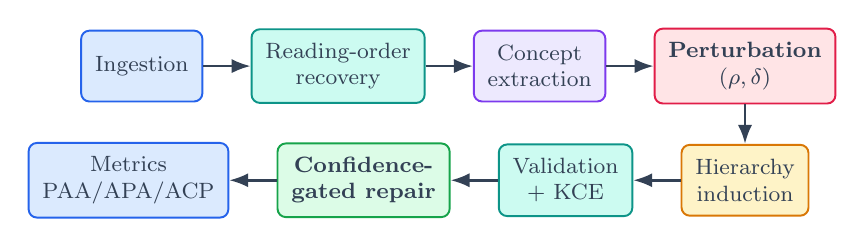
\begin{tikzpicture}[node distance=5mm and 6mm]
\node[stage,sBlue] (a){Ingestion};
\node[stage,sTeal,right=of a] (b){Reading-order\\recovery};
\node[stage,sViolet,right=of b] (c){Concept\\extraction};
\node[stage,sRose,right=of c] (p){\textbf{Perturbation}\\$(\rho,\delta)$};
\node[stage,sAmber,below=of p] (h){Hierarchy\\induction};
\node[stage,sTeal,left=of h] (v){Validation\\+ KCE};
\node[stage,sGreen,left=of v] (r){\textbf{Confidence-}\\\textbf{gated repair}};
\node[stage,sBlue,left=of r] (m){Metrics\\PAA/APA/ACP};
\draw[farrow](a)--(b);\draw[farrow](b)--(c);\draw[farrow](c)--(p);\draw[farrow](p)--(h);
\draw[farrow](h)--(v);\draw[farrow](v)--(r);\draw[farrow](r)--(m);
\end{tikzpicture}
\caption{Study pipeline. The recovered hierarchy is an instrument; the shaded blocks (perturbation
and confidence-gated repair) are the research contributions.}
\label{fig:pipe}
\end{figure}

\section{Instrument: Layout-Aware Structure Recovery}
The instrument ingests a PDF with pdfplumber, recovers reading order with a column-gutter rule
(blocks are split at the page gutter and sorted column by column with a vertical tolerance
$\tau_y=20$~pt), and classifies headings by section numbering or relative font size. Each heading
becomes a concept node grounded to its source block. Attachment is \emph{numbering-primary}: a
number such as ``3.1'' attaches to ``3''; unnumbered headings fall back to a Parent Ranking Engine
(PRE) that scores candidates by reading-order proximity, TF--IDF similarity~\cite{salton1983introduction}
and heading level. Every edge is validated by an upward DFS so the result is acyclic, single-parent
and depth-bounded, and each node receives a Knowledge Confidence Estimation (KCE) score propagated
in topological order via Kahn's algorithm~\cite{kahn1962topological}. This instrument is the author's
prior implementation and is reused unchanged.

\section{Perturbation Model}
Two independent error sources model real parser failure. Reading-order noise swaps each adjacent pair
of concepts in reading order with probability $\rho$. Heading-number dropout removes a heading's
section number with probability $\delta$, forcing the semantic PRE fallback for that heading. Both
are applied to copies of the extracted concepts, after which the hierarchy is rebuilt and re-scored.

\section{Retrieval-Relevant Metrics}
Let $\mathrm{gold}(c)$ be the parent of concept $c$ implied by its original numbering, and
$\mathrm{anc}(c)$ its gold ancestor chain to the root.
\begin{itemize}
  \item \textbf{PAA} $=$ fraction of nodes whose predicted immediate parent equals $\mathrm{gold}(c)$.
  \item \textbf{APA} $=$ fraction of nodes whose \emph{entire} predicted ancestor set equals
  $\mathrm{anc}(c)$; this is exactly the context a hierarchical retriever would attach.
  \item \textbf{ACP} $=$ mean over nodes of
  $|\widehat{\mathrm{anc}}(c)\cap\mathrm{anc}(c)| / |\widehat{\mathrm{anc}}(c)|$, the precision of the
  attached ancestor context.
\end{itemize}
No language model is used, so any change is attributable to structure alone.

\section{Confidence-Gated Repair}
Repair uses the existing KCE score as an error detector. For each non-root node $c$ with
$\mathrm{conf}(c) < \tau$, the predicted (possibly corrupted) parent is discarded and $c$ is
reattached to the nearest earlier heading of shallower level --- a safe structural prior --- as in
Algorithm~\ref{alg:repair}. The step needs no re-parsing of the PDF.

\begin{algorithm}[!htbp]
\caption{Confidence-Gated Structural Repair}\label{alg:repair}
\begin{algorithmic}[1]
\REQUIRE concepts in reading order, confidence threshold $\tau$
\FORALL{non-root concept $c$}
  \IF{$\mathrm{conf}(c) < \tau$}
    \STATE $u \leftarrow$ nearest earlier concept with $\mathrm{level}(u) < \mathrm{level}(c)$
    \STATE $\mathrm{parent}(c) \leftarrow u$ (or root if none)
  \ENDIF
\ENDFOR
\end{algorithmic}
\end{algorithm}

\section{Summary}
The methodology reuses a validated layout-aware instrument, corrupts its output in a controlled way,
scores the result with retrieval-relevant metrics, and repairs weak structure using the existing
confidence signal.

% ===================== CH4 WORK DONE =====================
\chapter{Work Done}

\section{Implementation and Experimental Setup}
The instrument is implemented in Python (pdfplumber, scikit-learn, NumPy, Pydantic). The new
perturbation harness, metrics and repair are implemented in a single evaluation module. Experiments
use a corpus of eleven real research-paper PDFs from the RAG literature (RAPTOR, GraphRAG, TreeRAG,
Self-RAG, HiChunk, RETRO, Atlas, T-RAG, REALM, HAT-RAG, and the original RAG paper); gold structure
is derived from section numbering. Every setting is averaged over five random seeds. No language
model is involved, isolating the structural effect.

\section{Degradation Under Structural Error}
Table~\ref{tab:deg} and Figure~\ref{fig:deg} report structural fidelity as each error source
increases. Reading-order noise has almost no effect (APA $96.8\%\rightarrow 96.4\%$ at $\rho=0.5$):
because attachment is numbering-primary, the section number encodes the parent independently of
order, so the hierarchy inherits robustness to reading-order errors. Heading-number loss degrades
fidelity steadily (PAA $97.7\%\rightarrow 92.7\%$, APA $96.8\%\rightarrow 89.2\%$, ACP
$97.3\%\rightarrow 91.2\%$ at $\delta=0.5$), because losing the number forces the weaker semantic
fallback. This confirms H1 for heading-number loss and reveals that the dominant vulnerability is
heading detection, not reading order.

\begin{table}[!htbp]\centering
\caption{Structural fidelity (\%) vs.\ heading-number dropout $\delta$ (mean over 11 documents, 5 seeds).}
\label{tab:deg}\renewcommand{\arraystretch}{1.2}{\small
\begin{tabularx}{\textwidth}{@{} >{\centering\arraybackslash}X *{6}{>{\centering\arraybackslash}p{1.4cm}} @{}}
\toprule
$\delta$ & 0.0 & 0.1 & 0.2 & 0.3 & 0.4 & 0.5 \\ \midrule
PAA & 97.7 & 96.3 & 95.1 & 94.7 & 93.8 & 92.7 \\
APA & 96.8 & 94.2 & 92.2 & 91.2 & 90.4 & 89.2 \\
ACP & 97.3 & 95.3 & 93.8 & 93.1 & 92.3 & 91.2 \\ \bottomrule
\end{tabularx}}
\end{table}

\begin{figure}[!htbp]\centering
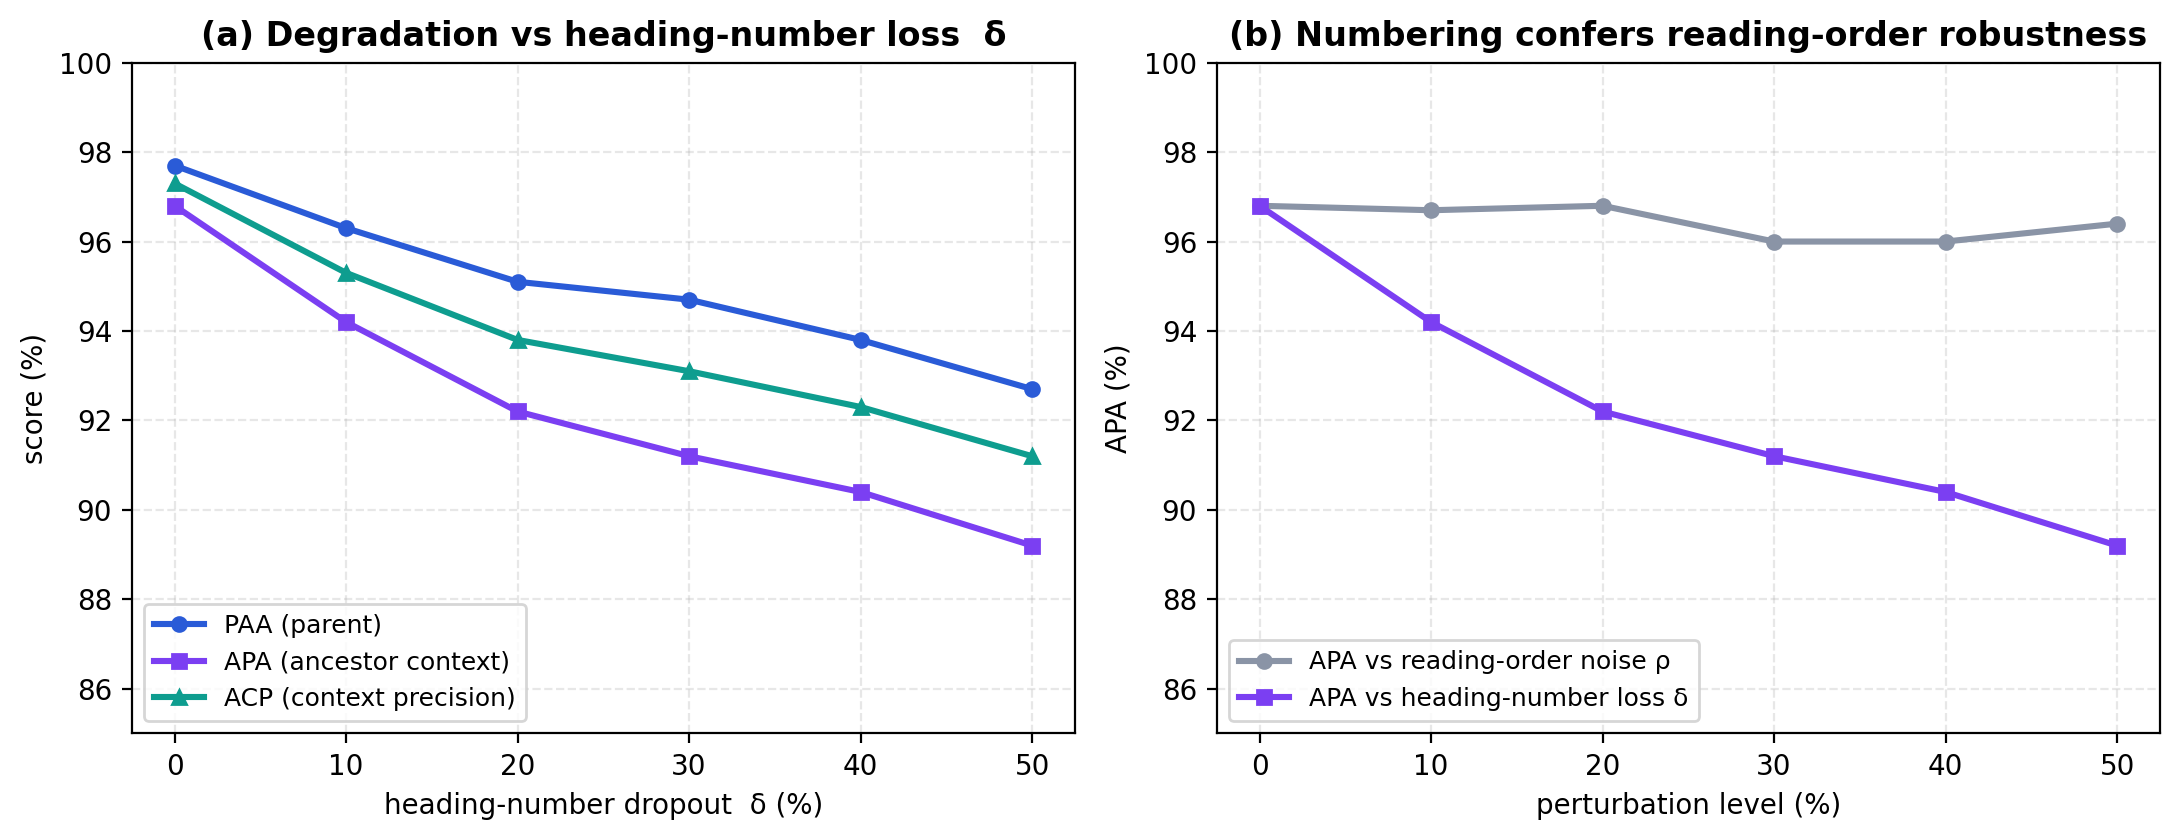
\includegraphics[width=\textwidth]{images/robustness_figure.png}
\caption{(a) Structural fidelity degrades steadily with heading-number loss $\delta$. (b) The same
hierarchy is almost unaffected by reading-order noise $\rho$, showing that numbering-primary
attachment confers reading-order robustness.}
\label{fig:deg}
\end{figure}

\section{Are Errors Predictable from Confidence?}
At $\delta=0.3$, correctly attached nodes have a mean KCE confidence of $0.611$ and wrongly attached
nodes $0.548$ (gap $+0.062$); the point-biserial correlation between confidence and correctness is
$r=+0.16$ over $980$ nodes. Confidence is therefore a real but weak predictor of attachment error
(partly supporting H2): the current heuristic KCE carries error information, but not strongly.

\section{Confidence-Gated Repair}
Table~\ref{tab:repair} shows the repair ablation at $\delta=0.3$, $\tau=0.60$. Gated repair improves
ancestor-context accuracy (APA $92.8\%\rightarrow 93.3\%$) and precision (ACP $94.1\%\rightarrow
94.4\%$). The gain is positive but small, and is bounded by the weak confidence signal: the repair
can only help where confidence correctly flags an error. This supports H3 while showing that the
value of the mitigation is limited by confidence quality.

\begin{table}[!htbp]\centering
\caption{Confidence-gated repair ablation at $\delta=0.3$, $\tau=0.60$ (mean over 11 documents, 5 seeds).}
\label{tab:repair}\renewcommand{\arraystretch}{1.25}{\small
\begin{tabularx}{\textwidth}{@{} X >{\centering\arraybackslash}p{2.2cm} >{\centering\arraybackslash}p{2.2cm} >{\centering\arraybackslash}p{2.2cm} @{}}
\toprule
Setting & PAA (\%) & APA (\%) & ACP (\%) \\ \midrule
No repair & 94.9 & 92.8 & 94.1 \\
Gated repair & \textbf{95.1} & \textbf{93.3} & \textbf{94.4} \\ \bottomrule
\end{tabularx}}
\end{table}

\section{Summary}
Across the corpus, reading-order noise is almost harmless while heading-number loss degrades the
retrieval context steadily; attachment errors fall on lower-confidence nodes; and a confidence-gated
repair recovers part of the loss. The size of the recovery is limited by the quality of the
confidence signal.

% ===================== CH5 CONCLUSIONS =====================
\chapter{Conclusions and Future Work}

\section{Conclusions}
This project gives the first robustness characterisation of structure-aware retrieval. Using a
controlled perturbation of a validated layout-aware pipeline and three model-free, retrieval-relevant
metrics, it shows that numbering-primary attachment is inherently robust to reading-order errors
(APA $\approx 96\%$ across all $\rho$), while heading-number loss degrades the ancestor context that a
hierarchical retriever would attach (APA $96.8\%\rightarrow 89.2\%$). Attachment errors concentrate
on lower-confidence nodes, and a confidence-gated repair recovers part of the loss without
re-parsing. The study turns a preprocessing pipeline into a research instrument and yields both a
design insight and an inference-time mitigation.

\section{Limitations}
\begin{enumerate}\setlength{\itemsep}{1pt}
  \item Fidelity is measured with structural proxies (PAA/APA/ACP), not end-task question answering.
  \item The confidence signal is a hand-crafted heuristic and only weakly predicts errors ($r\approx0.16$), which caps the repair gain.
  \item Gold structure is numbering-derived, so unnumbered-heading correctness is not directly graded.
  \item The corpus is eleven academic PDFs; non-academic layouts are untested.
\end{enumerate}

\section{Future Work}
\begin{enumerate}\setlength{\itemsep}{1pt}
  \item Replace the heuristic KCE with a \emph{learned} structural-confidence estimator to strengthen detection and repair.
  \item Add an LLM-in-the-loop evaluation to connect structural fidelity to answer quality and faithfulness.
  \item Extend perturbation to the block level (before heading detection) and to larger public document-QA corpora.
  \item Study robustness under heterogeneous and federated document sources.
\end{enumerate}
These directions form the objectives of the Major Project, of which this robustness study is the
first objective.

% ===================== REFERENCES =====================
\clearpage
\renewcommand{\bibname}{REFERENCES}
\phantomsection\addcontentsline{toc}{chapter}{REFERENCES}
\begin{thebibliography}{99}
\bibitem{lewis2020rag} P.~Lewis, E.~Perez, A.~Piktus, et al. Retrieval-augmented generation for knowledge-intensive NLP tasks. In \textit{NeurIPS}, vol.~33, pp.~9459--9474, 2020.
\bibitem{guu2020realm} K.~Guu, K.~Lee, Z.~Tung, P.~Pasupat, and M.~Chang. REALM: Retrieval-augmented language model pre-training. In \textit{ICML}, pp.~3929--3938, 2020.
\bibitem{borgeaud2022retro} S.~Borgeaud, A.~Mensch, J.~Hoffmann, et al. Improving language models by retrieving from trillions of tokens. In \textit{ICML}, pp.~2206--2240, 2022.
\bibitem{izacard2023atlas} G.~Izacard, P.~Lewis, M.~Lomeli, et al. Atlas: Few-shot learning with retrieval augmented language models. \textit{JMLR}, 24(251):1--43, 2023.
\bibitem{asai2024selfrag} A.~Asai, Z.~Wu, Y.~Wang, A.~Sil, and H.~Hajishirzi. Self-RAG: Learning to retrieve, generate, and critique through self-reflection. In \textit{ICLR}, 2024.
\bibitem{sarthi2024raptor} P.~Sarthi, S.~Abdullah, A.~Tuli, et al. RAPTOR: Recursive abstractive processing for tree-organized retrieval. In \textit{ICLR}, 2024.
\bibitem{tao2025treerag} W.~Tao, X.~Xing, Y.~Chen, L.~Huang, and X.~Xu. TreeRAG: Unleashing the power of hierarchical storage for enhanced knowledge retrieval in long documents. In \textit{Findings of the ACL}, pp.~356--371, 2025.
\bibitem{lu2026hichunk} W.~Lu, K.~Chen, R.~Qiao, and X.~Sun. HiChunk: Evaluating and enhancing retrieval-augmented generation with hierarchical chunking. arXiv:2509.11552, 2025.
\bibitem{bookrag2025} Y.~Zhang, et al. BookRAG: A hierarchical structure-aware index-based approach for retrieval-augmented generation on complex documents. arXiv:2512.03413, 2025.
\bibitem{ladrag2025} Z.~Xu, et al. LAD-RAG: Layout-aware dynamic RAG for visually-rich document understanding. arXiv:2510.07233, 2025.
\bibitem{wallat2025faith} J.~Wallat, et al. Correctness is not faithfulness in retrieval-augmented generation attributions. In \textit{ACM SIGIR ICTIR}, 2025.
\bibitem{ogorman1993document} L.~O'Gorman. The document spectrum for page layout analysis. \textit{IEEE TPAMI}, 15(11):1162--1173, 1993.
\bibitem{breuel2002high} T.~M.~Breuel. Two geometric algorithms for layout analysis. In \textit{Document Analysis Systems}, pp.~188--199, Springer, 2002.
\bibitem{huang2022layoutlmv3} Y.~Huang, T.~Lv, L.~Cui, Y.~Lu, and F.~Wei. LayoutLMv3: Pre-training for document AI with unified text and image masking. In \textit{ACM Multimedia}, pp.~4083--4091, 2022.
\bibitem{salton1983introduction} G.~Salton and M.~J.~McGill. \textit{Introduction to Modern Information Retrieval}. McGraw-Hill, 1983.
\bibitem{kahn1962topological} A.~B.~Kahn. Topological sorting of large networks. \textit{Communications of the ACM}, 5(11):558--562, 1962.
\end{thebibliography}
\end{document}
